\chapter{Procedimiento}
\label{ch:procedimiento}

En el desarrollo de este TFG se ha utilizado una metodología ágil basada en \emph{Scrum}~\cite{scrumguide}, definida por el director.  El trabajo se ha dividido en iteraciones de dos semanas denominadas \emph{sprints}.  Las unidades de trabajo se presentan en forma de historias de usuario (\emph{user stories}) que definen mini-proyectos de muy corta duración que aportan valor al proyecto.  Es decir, cada historia de usuario cumple o ayuda a cumplir alguno de los objetivos.  Medir el valor percibido corresponde al propietario del producto (\emph{Product Owner}), que participa activamente en la planificación del proceso priorizando las unidades de trabajo.

La utilización de una metodología ágil permite equilibrar la cantidad de trabajo y los objetivos alcanzados.  Los 12 créditos ECTS del TFG se reparten según el criterio del director para que los resultados aporten el máximo valor posible, incluso en presencia de imprevistos.

\section{Diferencias con Scrum}

\emph{Scrum} es una metodología estrictamente centrada en el cliente.  El cliente es el responsable de priorizar y, en cierto modo, planificar las iteraciones.  Esto garantiza que la ejecución del proyecto responde al máximo con las expectativas del cliente, aún cuando los imprevistos impidan alcanzar alguno de los objetivos iniciales.  Esta característica de \emph{Scrum} es la única que se ha intentado mantener inalterada.  Sin embargo, el TFG es un proyecto individual, lo que ha requerido modificar significativamente otros aspectos de la metodología.

\subsection{Roles}

La única remuneración que se obtiene con la ejecución de un TFG es la calificación de los distintos aspectos (anteproyecto, valoración del director, valoración del tribunal, etc.).  Por tanto, el cliente del TFG se compone por el director y el tribunal de la defensa.  Desgraciadamente no es posible conocer a priori el tribunal.  Por este motivo el director es el único representante del cliente en el proceso de desarrollo (\emph{Product Owner}).

El TFG debe ser realizado de manera individual.  Por tanto, el equipo de trabajo (\emph{Team Member}) se compone exclusivamente por el autor.

La labor de dirección del TFG se asimila a la de dirección del proyecto y, por tanto, el director también actúa como coordinador del proceso, o \emph{Scrum Master}.  Nótese que hay dos roles representados por la misma persona.  Desde un punto de vista purista esto implica que puede haber conflicto de intereses y los intereses del cliente pueden estar insuficientemente representados.  Es una limitación extrínseca, que no es posible solucionar con el proceso actual.  Aún así, el uso de una metodología ágil centrada en el cliente debe mejorar el alineamiento de intereses cuando sobrevienen problemas que afectan o pueden afectar a la consecución de alguno de los objetivos iniciales.

\subsection{Historias de usuario}

\emph{Scrum}, como la mayoría de los métodos ágiles, está enfocada al desarrollo de proyectos en entornos de alta incertidumbre por equipos multidisciplinares bien formados.  El desarrollo de un TFG, al tratarse de un primer proyecto profesional, también está sometido a gran cantidad de incertidumbre.  Sin embargo, no siempre se cuenta con la formación previa necesaria para abordar todos los problemas.  Esto implica que, en ocasiones, se necesita aprender o leer, sin repercusión medible en el valor percibido por el \emph{Product Owner}.  En esos casos se planifican unidades de trabajo que no corresponden estrictamente a historias de usuario en el sentido de Scrum.  Se ha intentado mantener al mínimo este tipo de historias de usuario para tener el proceso lo más controlado posible.

Puntualmente ha sido necesario planificar historias de usuario que solo pretenden explorar opciones.  Este tipo de historias de usuario están contempladas en \emph{Scrum}, se denominan \emph{spikes}.  Sin embargo, en la ejecución de este TFG se ha procurado reducir al mínimo para que la exploración de alternativas no domine en el tiempo dedicado al TFG.

\subsection{Planificación de sprints}

Para la planificación y el seguimiento se ha utilizado un tablero \href{http://trello.com}{Trello}.  Los tableros Trello permiten agrupar tarjetas en una serie de listas con nombre.  Se ha utilizado el esquema propuesto en~\cite{andrewlittlefield2018}.

El autor ha sido responsable de añadir la mayoría de las historias de usuario a la lista \emph{Backlog}.  Se trata de un proceso continuo, durante toda la ejecución del proyecto.  El director, como \emph{product owner}, prioriza las historias, moviendo las tarjetas dentro de la lista \emph{Backlog}.  Justo antes de cada iteración se realiza una reunión presencial o virtual para revisar la iteración pasada y planificar la siguiente iteración.

Usando la técnica de \emph{planning poker} (ver~\cite{scrumguide}) se dimensionan las historias de usuario en días de trabajo.  Esta técnica consiste en un proceso de generación de consenso entre el autor y el director sobre el tiempo requerido para la ejecución de cada historia de usuario.  La unidad empleada ha sido de un día.

El director, como \emph{product owner} traslada las tarjetas correspondientes a las primeras historias de la lista \emph{Backlog} a la lista \emph{ToDo} hasta completar los 10 días de trabajo de la iteración.

\subsection{Flujo de trabajo}

El flujo de trabajo diario del autor corresponde a la siguiente secuencia:

\begin{itemize}
    \item Dentro de la lista \emph{ToDo} puede elegirse cualquier tarjeta para trabajar en ella.  Antes de comenzar el trabajo se arrastra la tarjeta a la lista \emph{Doing}.  Esto proporciona información en tiempo real al director del progreso de la iteración.
    
    \item Al terminar una historia de usuario la tarjeta correspondiente se arrastra a la lista \emph{QC} (quality control).
    
    \item El director, como \emph{Scrum Master}, revisa que la historia está realmente acabada y, si así es, la traslada a la lista \emph{Done}. En caso contrario la traslada a la lista \emph{Doing} otra vez, añadiendo un comentario que lo justifica.

    \item Si en el transcurso del trabajo se encuentra un obstáculo que impide progresar con una historia, se traslada a la lista \emph{Blocked}, añadiendo un comentario que lo justifica.
\end{itemize}

En todo momento es posible ver el estado global de ejecución del proyecto.  Al finalizar, la lista \emph{Done} contiene todas las historias de usuario ejecutadas por orden de terminación.  Y las listas \emph{Blocked} y \emph{Backlog} contienen (en este orden) todas las historias de usuario que corresponderían a trabajo futuro, ya priorizadas por el director.

\subsection{Herramientas de ayuda}

El proceso de desarrollo está fuertemente ligado a la herramienta \href{https://trello.com/}{Trello}.  Se trata de una herramienta colaborativa en línea, que permite mantener una serie de tarjetas agrupadas en listas con nombre.  Cada tarjeta puede tener un título, una descripción, un conjunto de adjuntos, y un conjunto de comentarios.  Trello se ha usado con éxito en la planificación de proyectos de nivel de complejidad muy variable.  Por ejemplo, Epic Games utiliza un tablero Trello para planificar las características a incorporar a cada nueva versión de Unreal Engine.  Por otro lado, un problema de Trello es el manejo limitado de la historia de modificaciones en las tarjetas y en los movimientos entre listas de tarjetas.  Esto dificulta en cierto modo el seguimiento de los cambios y, sobre todo, la corrección de errores en el proceso.  Por este motivo, Trello solo se ha empleado en la coordinación del trabajo, mientras que toda la gestión de cambios se ha delegado en otra herramienta.

Todo el proyecto ha sido gestionado desde su inicio con una herramienta de control de versiones distribuido en un repositorio público de GitHub, disponible en \thegitrepo.  Cada vez que se completa con éxito una historia de usuario se notifica mediante un comentario en la tarjeta correspondiente.  Este comentario tan solo contiene el identificador del paquete de cambios (\emph{commit}) que da por concluida la historia.  Todos los \emph{stakeholders} pueden consultar la evolución del proyecto en todo momento desde la propia página del repositorio.

\begin{figure}[tbp]
\centering
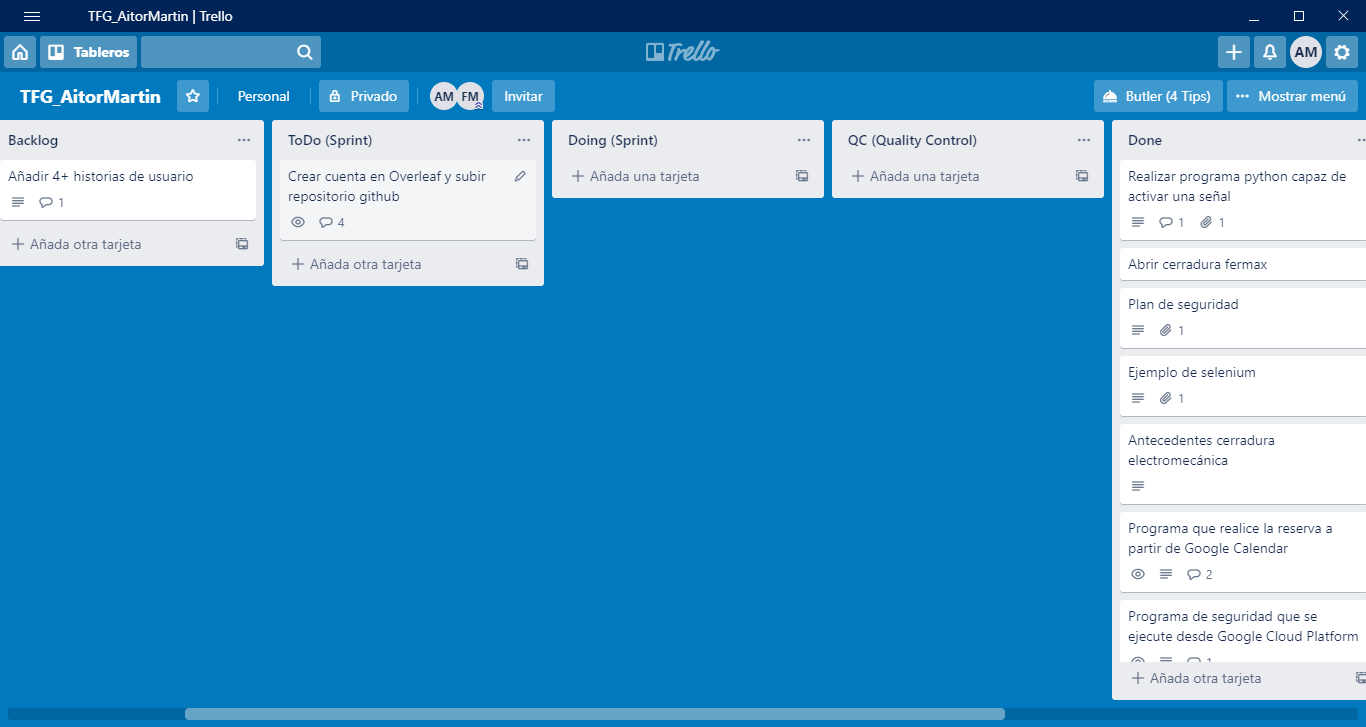
\includegraphics[scale = 0.4]{fig/tableto-trello.PNG}
\caption{Tableto trello utilizado en el desarrollo de este trabajo de fin de grado}
\label{fig:tableto-de-trello}
\end{figure}